\documentclass{article}
\usepackage[utf8]{inputenc}

\usepackage[margin=1in]{geometry} 
\usepackage{amsmath,amsthm,amssymb,scrextend}

	% Page Display
	\usepackage{url} % Allows for url links
	\usepackage{graphicx} % Allows for inputing figures
	\usepackage[dvipsnames]{xcolor} % For pretty colors

	% Math Typesetting
	\usepackage{amsmath} % Provides useful equation formats
	\usepackage{amssymb} % Provieds a ton of useful math symbols
	\usepackage{mathtools} % Provides patches for amsmath

	% TikZ/pgfPlots
	\usepackage{tikz}
	\usepackage{pgfplots}
	\pgfplotsset{compat=1.14}
	\usetikzlibrary{automata,arrows,positioning,calc}
	\pgfplotsset{ every non boxed x axis/.append style={x axis line style=-}, every non boxed y axis/.append style={y axis line style=-}}
	\usepackage{float}
	%\usepackage{caption}
	\setlength{\parindent}{0pt}
	\usepackage{xspace}
	\usepackage{expl3}
	\expandafter\def\csname ver@l3regex.sty\endcsname{} 
	\usepackage{coloremoji}

\title{Theta Model}
\author{Daniel Borrus}
\date{February 14th, 2020}


\begin{document}

\newcommand{\Iapp}{$I_{\text{app}}$ \xspace}
\newcommand{\Iappi}{$I_{\text{app}_i}$ \xspace}
\newcommand{\dskip}{\vskip 2mm}
\newcommand{\pre}{preB\:otC \xspace}
\renewcommand{\thefootnote}{\fnsymbol{footnote}}

\maketitle

\section{Introduction}
This is a network model of simple oscillators, here called neurons. 

% \begin{align}
%     \dot{\theta}_i &= \frac{1 - \cos{\theta_i} + [1+\cos{\theta_i}] I_{\text{app}_i}}{\theta_\tau} \\
%     \dot{m}_i &= -m_i/m_\tau \\
%     \dot{n}_i &= \alpha_n m_i (1-n_i) - n_i/n_\tau \\
%     \dot{s}_i &=-s_i/s_\tau
% \end{align}
%
\vskip 2mm
\noindent
Consider a network of $N$ neurons. The phase of a given neuron, $i$, in the network of $N$ neurons is given by $\theta_i$, where
\begin{equation} \label{thetaODE}
    \dot{\theta}_i = \frac{1 - \cos{\theta_i} + [1+\cos{\theta_i}] I_{\text{app}_i}}{\theta_\tau}.
\end{equation}
See the phase diagram of the ODE below, to quickly understand the behavior.
\begin{figure}[h!]
\centering
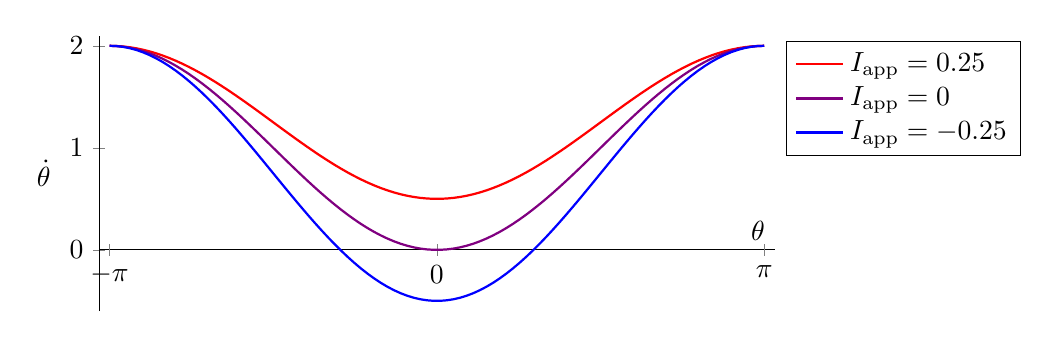
\begin{tikzpicture}
\begin{axis}[height = 2in,
		   width = 4in,
		   axis x line = middle,
		   axis y line = left,
		   xlabel = $\theta$,
		   ylabel = $\dot{\theta}$,
		   ylabel style = {rotate=-90},
		   xmin = -pi-.1,
		   xmax = pi+.1,
		   ymin=-0.6,ymax=2.1,
		   xtick = {0},
		   extra x ticks = {-pi,pi},
		   extra x tick labels = {$-\pi$,$\pi$},
		   legend entries = {$I_{\text{app}}=0.25$,$I_{\text{app}}=0$,$I_{\text{app}}=-0.25$},
		   legend style = {xshift=1.3 in},
		   legend cell align={left},
		   ]
		   \plot[red,thick,domain=-pi:pi,samples=100] {1-cos(deg(x)) + (1 + cos(deg(x))) * 0.25};
		   \plot[red!50!blue,thick,domain=-pi:pi,samples=100] {1-cos(deg(x)) + (1 + cos(deg(x))) * 0};
		   \plot[blue,thick,domain=-pi:pi,samples=100] {1-cos(deg(x)) + (1 + cos(deg(x))) * -0.25};
\end{axis}
\end{tikzpicture}
\caption{Plot of Equation \ref{thetaODE} with two different $I_{\text{app}}$. $\theta_\tau = 1$} \label{fig:1}
\end{figure}

When a neuron $\theta_i$ crosses $>\pi$ it ``fires'' and is reset back to $-\pi$. As the ODE has a period of $2\pi$, the dynamics are unaffected. As one can see from the phase diagram above, when \Iapp is negative, the neuron will be silent; when \Iapp is positive, the neuron will fire tonically.
\vskip 2mm
A neuron $i$ also has 3 additional ODEs, and probably 1 additional state variable. $m_i$ and $n_i$ describe the synaptic depression of a given neuron $i$, where ultimately the synaptic depression is $y=1-n$.
\begin{align}
    \dot{m}_i &= -m_i/m_\tau \\
    \dot{n}_i &= \alpha_n m_i (1-n_i) - n_i/n_\tau
\end{align}
\vskip 2mm
After a burst ($\theta_i>\pi$), $m_i$ is stepped up a fraction of the way from its current value to $m=1$; the magnitude of this step is proportional to $m_\text{gain}$. Thus if a neuron ``spikes'' at time $t$, then
\[m_i(t+1) = m_i(t) + m_\text{gain}(1-m_i(t))\].
\vskip2mm
The variable $n$ rises more slowly, growing proportional to $m$. Thus synaptic depression comes on more gradually after a spike, and will grow with more rapid spiking, or activity. This allows synaptic depression ($y=1-n$) to move on a slower time-scale than the next term, synaptic conductance ($s$).

\vskip 2mm
The variable $s_i$ describes the amount of synaptic current a neuron generates for downstream neurons. It's behavior is simple,
\begin{equation}
    \dot{s}_i =-s_i/s_\tau
\end{equation}
But similar to $m_i$, after a spike $s_i$ immediately increases an amount proportional to $s_\text{gain}$ so that
\[s_i(t+1) = m_i(t) + s_\text{gain}(1-s_i(t))\]. So after a spike, a neuron generates an ``EPSP'' that decays away with rate $s_\tau$.

\vskip 2mm

Ultimately, synaptic depression ($y$) and conductance ($y$) determine the amount of ``current'' an upstream neuron generates for its target neurons. For each time step, a neuron's \Iappi is calculated as
\begin{equation}\label{Iapp}I_{\text{app}_i} = I_0 + d\sum_j s_j y_j\end{equation}
where $I_0$ is the intrinsic \Iapp for each neuron (this can be the same for every neuron, or a distribution). $d$ is the strength of the synaptic connection, a scalar. $s_j$ is the synaptic conductance for all upstream neurons $j$ from neuron $i$. $y_j$ is the synaptic depression for all upstream neurons $j$ from neuron $i$. Thus, Equation \ref{Iapp} reads: The applied current a neuron $i$ receives at any time step is equal to an intrinsic applied current ($I_0$), plus the strength of all upstream neuron synapses (a product of their synaptic conductance ($s_j$) and recovery from synaptic depression ($y_j$)). 

\section{Network}
An important question that we are very interested in is what the network topology should be. For the purpose of this short overview of the model, I will focus on two network structures.

\dskip

The network structure we were using was an Erdos-Renyi random network with connectivity of $p=0.14$. It's worth pointing out, that for a network of 650 neurons, an ER network with $p=0.14$ leads to $91$ connections per node. A bit much. Regardless, a network like this can produce robust oscillations. See section \ref{examplesections}.

\dskip
The next network I want to discuss is the 2-d lattice described in \dskip
\texttt{Guerrier, Claire, John A. Hayes, Gilles Fortin, and David Holcman. “Robust Network Oscillations during Mammalian Respiratory Rhythm Generation Driven by Synaptic Dynamics.” Proceedings of the National Academy of Sciences 112, no. 31 (August 4, 2015): 9728–33. https://doi.org/10.1073/pnas.1421997112.}

\section{Simulation examples and network study}\label{examplesections}
Let's begin with the vanilla version of the model, with the ER network. The model is able to generate rhythmic bouts of spiking, where a single node spikes multiple times during a network-wide burst of activity. The neurons all have negative \Iappi, and are thus normally silent. Noise drives some of the nodes over threshold, and they begin to spike. This activity propagates throughout the network RAPIDLY and drives the upstroke of a burst. Synaptic depression begins to accumulate and the diminishing \Iapp terminates the burst. Synaptic depression must recover to some degree before another burst is possible. This last point, about recovery of synaptic depression and timing of the next burst, is an important one.


The model works in two different configurations. In one (with higher noise and slightly slower synaptic recovery), synaptic depression is not allowed to recover back to $y=1$ before the next burst is initiated. See the figure below. 
\begin{figure}[H]
\centering
\includegraphics[scale=.15]{highnoise_recoverystartsburst2.png}
\end{figure}
In the top row, we see network activity, and below that a raster plot. But focus on the third row: the mean synaptic depression of the entire network. Notice it is not fully recovered before the next spike. As a result, the size of the following burst will be proportional to the duration of the preceding inter-burst interval [CITE]. I've tested this in the model myself, and do find this relationship. This dependency of burst size on preceding interval is not observed in the \pre. And it has also been shown for the respiratory rhythm that synaptic depression appears to recover completely in the first half of the inter-burst interval [CITE]. So the above configuration of the network must be incomplete.
\dskip



In the second configuration synaptic depression is allowed to recover, now noise drives the network to burst. But we can quickly see the network is behaving strangely. The problem is with the inter-event intervals. We find the intervals are exponentially distributed. This is because we are waiting for a random event that has some probability of happening at any given time step. Specifically, we are waiting for noise to drive us above some threshold. After waiting 5 minutes for a burst or an hour, the burst is not any more likely at the next moment. This behavior is also inconsistent with the real \pre rhythm. So what gives!!?
\begin{figure}[H]
\centering
\includegraphics[scale=.15]{look at whats causing the burst.png}
\end{figure}
\dskip

Well what if we were no longer waiting for a time-independent event, but a time-dependent one. An event that became more likely the longer you waited for it. It's possible that ``a build up of excitability'' in the network could take several seconds, or the second half of the inter-event interval. But the question is, ``how much excitability can a dynamic network store?''


\section{Where to store excitability in a network}

% \subsection{synaptic conductance $s$}
% The dynamics of $s$ are meant to represent synaptic conductance, generated in the form of EPSPs. The excitatory drives last for some duration, and then decay away. Prolonging their duration, by increasing $s_\tau$ will keep ``excitation'' in the network. However, we should keep in mind biologically realistic boundaries for EPSP size and duration.
% It's also possible that prolonging EPSPs will just increase the bursting frequency

\subsection{Network Topology}
Our hypothesis is, under different network topologies, excitation can build and propagate through the network more slowly, and simply delay the network-wide burst that is inevitable. First, I looked to see at what rate the {\bf giant component }comes online for different networks. The results were surprising. I will show two important examples here.

First, I build a network with some desired properties. Then I take all the nodes of the network offline. Next, one at a time, I reinstall a node and all its outgoing edges. After I add a node, I recalculate the largest component in the directed\footnote{The definition of the giant component in a {\bf directed} graph requires more rigorous definition. The giant component we refer to here is the largest group of strongly connected components. In other words, if you start at node A, how many nodes can you pass through and still arrive back at A.}
network. 

Here is the result of this study for the ER network with $p=0.14$:

\begin{figure}[H]
\centering
\includegraphics[width=6in,height=2in]{Er3.png}
\end{figure}

\dskip

The size of the largest cluster (in blue) almost perfectly tracts the unity line $y=x$. That tells us, that anytime you add a random node into the network, it will likely already be a part of the giant component. This suggests there is minimal sub clustering of nodes. There are no secrets in the ER network of $p=0.14$.

What about other networks? Well one of the most extreme networks I found, when it comes to a giant component ``coming online'', was from Guerrier 2015 [Real citation]. There network is built on a 2-D lattice, where connections between neighbors ir proportional to their absolute distance. For the math inclined, the probability of node $i$ (at location $(x_i,y_i)$) connecting to node $j$ (at location $(x_j,y_j)$)is
\begin{align}
P_{i\rightarrow j}&=e^{-d^2/(2s^2)} \\
&\text{where} \nonumber \\
d &= \sqrt{(x_i-x_j)^2+(y_i-y_j)^2} \nonumber
\end{align}
In there case, $s=0.9$, which leads to a mean in/out degree of $<k_\text{in/out}> \approx 3.9$\footnote{compare that to the ER network with 90 average connections.}.

\end{document}
